\section{Milepæl 2}
\subsection{Introduksjon}
I denne milepælen har vi fokusert på å designe og implementere School-performance datasettet opp mot KV-store. Grunnen til at dette settet passer utmerket til KV er fordi vi ønsker å ha god fleksibilitet på dataen. Fleksibilitet og konsistens blir de viktigste aspektene for dette settet da det vil falle seg naturlig at elever slutter og starter på skolen, det gjennomføres nye prøver, eller fritids-situasjonen til elever kan endre seg. Siden dataen som måles er såpass lite rigid av seg selv, er det da en fordel at det lett kan gjøres endringer, legge til ny data, eller fjerne data. Disse tilfellene vil føre til at konsistens blir viktig da forskjellige personer skal kunne ha tilgang til å endre data, og hyppige endringer må kunne sjekkes mot tidligere versjoner.

Datasett: https://www.kaggle.com/larsen0966/student-performance-data-set/version/2

\subsection{Hvordan kommer data inn?}
Databasen vi har valgt tar utgangspunktet i et datasett som bruker data fra en undersøkelse på studenter fra to skoler i Portugal. For at ny data skal bli lagt inn i databasen, må det gjøres enda en undersøkelse ved enten de samme skolene eller en ny skole. Dataen må deretter legges inn via nettskjemaet med følgende felt på nettsiden:

\begin{itemize}
  \item Skole
  \item Kjønn
  \item Alder
  \item Mors-utdanning
  \item Fars-utdanning
  \item Reisetid
  \item Studietid
  \item Stryk
  \item Skolestøtte
  \item Ekstratimer (Betalt)
  \item Aktiviteter utenom faget
  \item Internett
  \item Romantisk forhold
  \item Familie Relasjon
  \item Fritid
  \item Gå ut med venner
  \item Alkohol i ukedagene
  \item Alkohol i helgen
  \item Helse
  \item Fravær
  \item Karakter semester 1
  \item Karakter semester 2
  \item Sluttkarakter
\end{itemize}

Totalt er det 22 felt som må fylles ut, men når dette er sagt kommer mange av feltene til å ha standardverdier. I tillegg til nettskjemaet vil det være mulig å laste opp datasett i form av CSV eller JSON som har de samme kolonnene. Rader som er duplikater, vil ikke bli tatt hensyn til siden det er mulig å produsere de samme verdiene. Dette vil si at noen må manuelt legge til data via nettsiden for at dataen skal dukke opp i databasen, den vil ikke lytte etter endringer i datasettet via API-er.

\subsection{RIAK eller ETCD}
I prosjektet vårt har vi bestemt oss for å bruke ETCD, siden ETCD prioriterer konsistensen til dataen over tilgjengelighet. Dette er viktig, siden for dette prosjektet er det mye viktigere at dataen stemmer, enn å ha rask respons-tid. Hele hensikten med denne seksjonen er å forstå effekten studenters bakgrunn har på resultatene ved de forskjellige skolene, derfor må dataen være oppdatert. Siden CAP-teoremet gjelder i praksis kun når det oppstår en nodefeil, betyr det ikke at vi ofrer tilgjengelighet fullstendig, men det er mindre viktig i dette tilfellet enn konsistens. Til slutt er det merkverdig å nevne at Riak er mye mer omfattende enn ETCD, derfor blir det også foretrukket i prosjektet.

\subsection{Design av nøkkel}
På grunn av måten vi velger å oppdatere eksisterende data i databasen, blir nøklene designet på en måte som skiller mellom komponenter og ny studentdata. Komponentene er JSON-objektene som brukes til å vise data på nettsiden, mens studentdataen er rådata som er nyttig for å holde dataen oppdatert. Hvis en student legges til eller oppdateres, oppdateres også komponentene i databasen. Den generelle strukturen på nøkkelen vil derfor være et prefiks for inndeling, etterfulgt av kolon, etterfulgt av navn eller id.

Verdier relatert til komponenter vil ha en nøkkel med prefiks "component" etterfulgt av navnet på komponenten. Eksempel på en nøkkel for en komponent i vår KV-store:

  component:studentByFreeTime


Verdier relatert til studenter vil ha nøkler med prefiks "student" etterfulgt av en 8-sifret id av typen Integer. Eksempel på en nøkkel for en student i vår KV-store:

  student:02381225

KV-store vil dermed følge en lignende struktur:


\begin{figure}[H]
  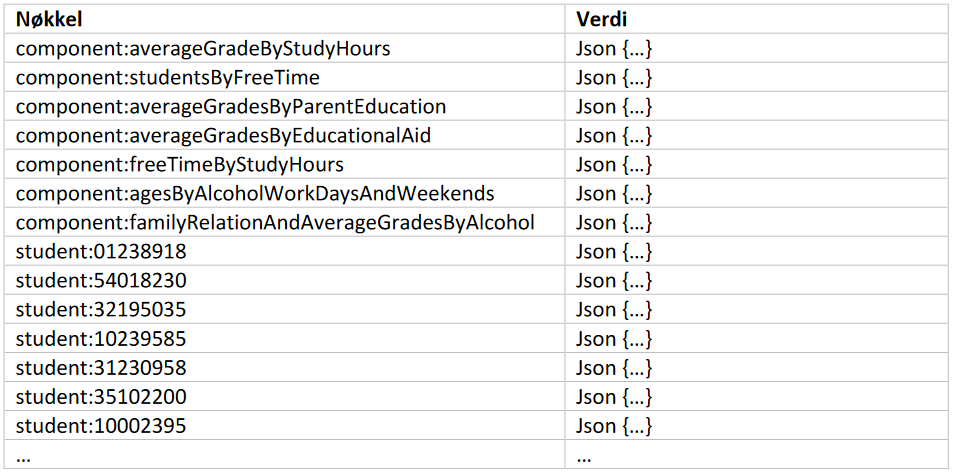
\includegraphics[width=\textwidth]{images/milepael2/tabellKVStore.png}
\end{figure}

\subsection{Design av dataobjekter og aggregeringer}
Som tidligere nevnt har vi delt opp dataobjektene i to grupper: komponenter og student-data. Grunnen til denne oppdelingen er for å optimalisere ytelse ved uthenting og oppdatering av data. Oppdelingen gjør det mulig å oppdatere individuelle komponenter ved å kun lese fra student-dataen som endret seg. Da unngår man å hente alle student-dataene for å oppdatere alle komponentene, og som resultat bruker nettsiden mindre kall til databasen.

\subsection{Ytelse og oppdatering av data}
På grunn av konsistens-kriterier for vår data, må read-kallene gjøres lineært som vil ta mer tid enn serialiserte kall. Ofte vil vi kun bruke et kall for å hente ut data, og heller bruke ytelsen til systemet for operasjoner på denne dataen.

En av grunnene til at dataen vil være lett tilgjengelig med få kall, er at den ikke nødvendigvis vil endre seg ofte (mange endringer heller i et kort tidsrom), men det er aggregeringene som gjøres med dataen som tar lang tid. Derfor er konsistens på dataen mye viktigere. Vi er avhengig av at dataen er korrekt og blir sjekket mot klyngen mer enn at uthenting av ny data er rask.

Ved første innlastning av nettsiden må den gjøre noen kall til databasen slik at den kan vise data på nettsiden. Siden det er 7 komponenter i denne nettsiden, har vi valgt å lagre hver komponent for seg i KV-store. Grunnen til dette er fordi hver komponent er ganske omfattende, og vi vil heller gjøre noen ekstra kall enn å laste et stort dataobjekt for hver oppdatering. Derfor blir det umiddelbart 7 kall mot KV-store når siden lastes inn.

Dersom vi ikke hadde designet dataen på denne måten, ville vi støtet på et problem dersom kun noen få studenter oppdateres. For eksempel med "averageGradesByStudyHours" komponentet i et datasett med 100 studenter, der 1 student endret verdi:

\begin{itemize}
  \item Hente alle studentobjekter fra databasen
  \item Bygge et averageGradesByStudyHours objektet på nytt
  \item Oppdater averageGradesByStudyHours i KV-store med den nye versjonen
  \item Oppdater studenten i KV-store med den nye versjonen
\end{itemize}

Det første steget ville bruke 100 kall, en for hver student, det tredje og fjerde steget er to kall. Til sammen blir dette 102 kall. Men siden vi har strukturert databasen ettersom, vil vi kunne minske dette tallet betraktelig. Med samme eksempel som over, her er måten vi gjør det på:

\begin{itemize}
  \item Hente gammelt student-objekt fra KV-store
  \item Hente komponent med key=component:averageGradesByStudyHours
  \item Oppdatere dataen i komponentet i koden ved å gjøre beregninger
  \item Lagre oppdatert komponentet i KV-store
  \item Lagre oppdatert student-objekt i KV-store
\end{itemize}

Steg 1, 2, 4 og 5 gjør 1 kall hver, som betyr at her gjør vi kun 4 kall mot KV-store. Denne metoden vil også brukes for å oppdatere de resterende komponentene, som betyr at hver oppdatering er kun 4 kall.

Det er viktig å punktere at samme metode vil også bli brukt dersom man oppdaterer data ved å laste 
opp en ny CSV fil. Den eneste forskjellen her er at programmet må først dekonstruere CSV-en for å hente innholdet før man gjør kall mot databasen.

\subsection{Hva om vi er dataeier?}
Den største forskjellen for produktet vårt ville vært hvor korrekt dataen er, hvem som hadde kunne gjort endringer, og hvordan/når de endringene ville blitt gjort. Nå kan det legges til eller endres når som helst, og det brukes verdier som ikke helt passer opp mot verdier vi heller er vant med, eller verdier som ikke er dekker hele spekteret vi ser etter (foreldreutdanning skulle gjerne hatt 3 ekstra verdier for bachelor/høyere utdanning, master, og phd. f.eks.).

Datasettet hadde mest sannsynlig da sett noe annerledes ut, og vært tilpasset våre behov. Dette betyr i hovedsak noe sammenslåing av kolonner, samt verdi endringer fra strenger til tall, eller andre grupperingsmetodikker.

Siden dette er forskning/spørreundersøkelser og data som skal hentes inn fra sikre kilder, men i større volum av gangen, ville det da heller vært logisk å laste hele csv-filer av gangen kontra slik som det vil være nå som man kan legge inn en og en student i nettskjemaet. Selvfølgelig ville det også vært mulig dersom datasett endrer seg, men hele datasettet ville nok blitt lastet på nytt med sjekker om oppdatert data.

Vi ville fremdeles ikke byttet til RIAK da dataen vi har er mest avhengig av konsistens, og trenger ikke noen spesielt høy grad av tilgjengelighet. Pga. dette vil lineære lese-spørringer i ETCD være bedre enn serialiserte spørringer i RIAK.

\subsection{Dataobjektene}
Denne seksjonen viser fram de forskjellige komponentene/dataobjektene med tilsvarende Json objekt og representasjon på nettsiden. Dette er for å illustrere hvordan vi ønsker at dataobjektene skal se ut. For hvert dataobjekt Vil det stå beskrevet hvordan data aggregeres, samt pseudo-kode på hvordan dataen hentes ut.

\subsubsection{Rådata}
\txt{code/milepael2/rawObject.json}
Dette dataobjektet er en en-til-en representasjon av en rad i datasettet og representerer en student.

\subsubsection{Dataobjekt 1}
\txt{code/milepael2/averageGradesByStudyHours.json}
Dette dataobjektet tar for seg den gjennomsnittlige karakteren for begge kjønn etter hvor mange timer de studerer i uken. Det er representert som et søylediagram i nettsiden. Her samler vi 4 grupper, en for hver tidsbergening, som hver splittes i to basert på kjønn, så regnes snitt-karakter.

\subsubsection{Dataobjekt 2}
\txt{code/milepael2/studentsByFreeTime.json}
Her viser dataobjektet prosentvis hvor mye fritid studentene har. Studenter grupperes etter hvor mye fritid de har, henter kun ut hvor stor hver gruppe er, så regnes 
det ut hvor stor hver gruppe er av totalen og prosent-verdien deres vises.

\subsubsection{Dataobjekt 3}
\txt{code/milepael2/averageGradesByParentEducation.json}
Denne grafen tar for seg et dataobjekt som samler mors og fars utdanningsnivå og viser karakterene barna har. Her hentes studentenes karakterer ut og legges inn i en gruppe for mors utdanningnivå, og en gruppe for fars, så snittes karakterene innad i disse gruppene.

\subsubsection{Dataobjekt 4}
\txt{code/milepael2/freeTimeByStudyHours.json}
Dette objektet viser hvor mye fritid studenter har i forhold til hvor mye de studerer. I dette dataobjektet må vi hente ut studenter i grupper etter hvor mye de jobber med skole på egen tid, og finner gjennomsnittet av hvor mye fritid de har på skalaen.

\subsubsection{Dataobjekt 5}
\txt{code/milepael2/familyRelationsAndAverageGradesByAlcohol.json}
Dataobjektet viser hvor mye alkohol en student drikker(delt etter helg og hverdag), hvordan forholdet studenten har til familien sin er, og hvordan dette påvirker karakterene i gjennomsnitt. I dette objektet henter vi ut grupper på lignende måte som i dataobjekt 6. Vi skaper da også 5 hovedgrupper med 2 subgrupper hver, en for helg og en for ukedag, og i hver av disse gruppene legges karakter og familie forhold inn og det utregnes gjennomsnitt. 

Denne aggregeringen vil ha mange operasjoner og vil være treg, men dataen har ikke noe særlig krav om å være lett tilgjengelig, eller at den må lastes spesielt fort, da det heller er viktig at dataen er korrekt.

